% functions:x18 GDC:NO
\begin{question}
  \hspace*{\fill} [Note Maximale: ?]\par
  \noindent Soit la fonction $y = a\,sin\,2x + c$, $-180 \le x \le 180$; $x$ est mesuré en degré.\par
  \medskip
  \begin{center} % or flushleft or flushright
    \noindent La courbe de la fonction est représentée ci-dessous.\par
    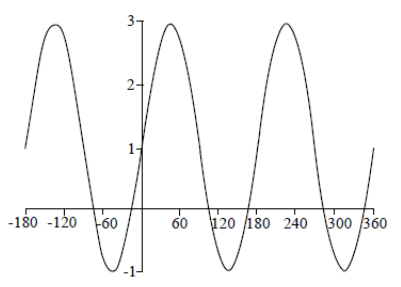
\includegraphics[scale=0.4]{figure_x18a}\par
    \noindent Figure A\par
  \end{center} % or flushleft or flushright

  \begin{enumerate}[label=(\alph*)]
    \item Donnez:
      \begin{enumerate}[label=(\roman*)]
        \item la période de cette fonction;\hspace*{\fill} [?] % optionally omit this mark and let the last sub-item be the sum of the sub-items
        \item l'amplitude de cette fonction.\hspace*{\fill} [?]
      \end{enumerate}
    \item Déterminez les valeurs de $a$ et de $c$.\hspace*{\fill} [?]
    \item Calculez l'abscisse x de la première intersection de la courbe avec la partie negative de l'axe
des abscisses.\hspace*{\fill} [?]
  \end{enumerate}
\end{question}
